\documentclass[11pt]{article}
\usepackage[margin=1in]{geometry}
\usepackage{amsmath,amssymb}
\usepackage{booktabs}
\usepackage{graphicx}
\usepackage{hyperref}
\usepackage{tikz}
\usepackage{pdflscape} % in preamble
\usetikzlibrary{arrows.meta,shapes.geometric,positioning,fit,calc}
\usepackage{algorithm}
\usepackage{algpseudocode}
\usepackage{xcolor}
\usepackage{caption}
\usepackage{enumitem}
\setlist[itemize]{noitemsep,topsep=2pt}
\setlist[enumerate]{noitemsep,topsep=2pt}
\usepackage{fontspec}




\title{\\ Homograph Disambiguation in NMT for Low-Resource Languages\\(TATN — Tri-Modal Adversarial Transparency Network)}

\date{}

\begin{document}
\maketitle



\bigskip

\section{Topic: title and description}
\textbf{Title:} \emph{Homograph Disambiguation in Neural Machine Translation for Low-Resource Languages.}

\textbf{Brief description}  
The research investigates methods to detect and resolve homographs (words with multiple distinct senses) in neural machine translation (NMT) for low-resource language pairs (example: Bengali $\rightarrow$ English). The proposed solution augments an encoder–decoder NMT with three cooperating modules:\\ \textbf{DSCD} (to detect ambiguous tokens and maintain online sense prototypes),\\ \textbf{ASBN} (to adversarially remove shortcut/spurious cues so the model relies on real contextual evidence), and\\ \textbf{TRG} (to generate and verify human-readable rationales for sense choices). Together these modules improve disambiguation accuracy and produce faithful explanations for decisions, which is especially valuable in low-resource settings where model overfitting to frequency is common.

\section{Three main components of TATN}

TATN integrates three modules. Below each module is described with its subparts, formulas, purpose, and interaction with other modules.

\subsection{DSCD — Dynamic Span–Sense Co-Detection}
\paragraph{Purpose.} Detect tokens or spans needing disambiguation, estimate their sense distribution, maintain online sense prototypes, and output multi-source uncertainty that drives both ASBN (adversarial strength) and TRG (rationale extraction).

\paragraph{High-level steps / parts}
\begin{itemize}
  \item \textbf{Buffers and prototype store}: per-surface-type circular buffer $B_w$ and prototype list $C_w=\{c_{w,1},\dots,c_{w,K_w}\}$. Buffers collect recent encoder vectors for type $w$; prototypes are centroids representing learned senses.
  \item \textbf{Type-level dispersion $D_w$}: measure of contextual variance across $B_w$. If $D_w > \delta_{\text{type}}$ mark type as candidate for multi-sense handling.
    \[
    \bar h_w = \frac{1}{|B_w|}\sum_{x\in B_w} x,\qquad
    D_w = \frac{1}{|B_w|}\sum_{x\in B_w} \|x - \bar h_w\|^2.
    \]
  \item \textbf{Per-token sense distribution}: compute cosine similarity to prototypes and softmax with temperature $T$:
    \[
    s_{j,i}=\frac{h_j^\top c_{w,i}}{\|h_j\|\|c_{w,i}\|},\qquad
    p_{j,i}=\frac{\exp(s_{j,i}/T)}{\sum_k\exp(s_{j,k}/T)}.
    \]
  \item \textbf{Predictive uncertainty (multi-source)}:
    \begin{itemize}
      \item \emph{Entropy} $H_j=-\sum_i p_{j,i}\log(p_{j,i}+\epsilon)$.
      \item \emph{MC-dropout variance} $\mathrm{Var}_j$ from $M$ stochastic passes.
      \item \emph{Aleatoric / $\sigma$-Net} $\sigma_j=\exp(\tfrac12 u_j)$ where $u_j=W_\sigma h_j+b_\sigma$.
      \item \emph{Novelty} $d_{\min}=\min_i (1-s_{j,i})$.
    \end{itemize}
    These combine into a single scalar $U_j$ (additive default, or normalized/weighted sigmoid form for fine control).
  \item \textbf{Dynamic clustering / prototype maintenance}:
    \begin{itemize}
      \item Track rolling assignment distances (mean $\mu_w$, std $\tau_w$).
      \item Adaptive creation threshold $\varepsilon_{\text{new},w}=\mu_w+\lambda \tau_w$.
      \item If $d_{\min}>\varepsilon_{\text{new},w}$ (and optionally $U_j>\delta_{\text{inst}}$) create new prototype $c_{w,K_w+1}\leftarrow h_j$ (cap with $K_{\max}$), else assign to nearest and update centroid via EMA:
      \[
      c_{w,i^\star}\leftarrow(1-\eta)c_{w,i^\star}+\eta h_j.
      \]
      \item Optionally require $N_{\min}$ assignments before a prototype is stable.
    \end{itemize}
  \item \textbf{Span detector and gating}: span head $\hat b_j=\sigma(W_{\text{span}}h_j+b_{\text{span}})$ and an attention gate $g_j=\sigma(w_g(U_j-b_g))$; the gate controls attention boosting and ASBN strength.
  \item \textbf{Sense-augmented embedding}: for flagged tokens, augment encoder vector with centroid:
    \[
    h'_j = h_j + c_{w,\hat y_j}.
    \]
\end{itemize}

\paragraph{Why DSCD is important}
DSCD provides explicit sense signals and a numeric uncertainty estimate that tells the system \emph{which} tokens need special handling. Prototypes act as interpretable, stored senses; uncertainty prevents overconfident wrong edits and guides TRG and ASBN in a targeted way. DSCD is particularly useful for low-resource languages because it builds sense anchors online and does not require large annotated sense inventories.

\subsection{ASBN — Adversarial Sense-Balance Network}
\paragraph{Purpose.} Prevent the model from exploiting spurious shortcuts (frequency, shallow context patterns, or alignment leakage) to resolve homographs. It does so with token-level adversarial discriminators applied through Gradient Reversal Layers (GRL) with per-token strengths determined by DSCD signals.

\paragraph{High-level parts}
\begin{itemize}
  \item \textbf{Discriminators} — specialized auditors:
    \begin{itemize}
      \item $D_{\text{freq}}$: detects frequency-based shortcuts (i.e., predicts the high-frequency surface→sense mapping).
      \item $D_{\text{ctx}}$: detects weak-context cues.
      \item $D_{\text{xl}}$: detects cross-lingual alignment leakage or target-side cues.
    \end{itemize}
  \item \textbf{Per-token GRL strength} (key innovation):
    \[
    \lambda_{k,j}=\operatorname{clip}\big(\bar\lambda_k\cdot p_{\max}(j)\cdot(1-U_j)\cdot g_j,\;0,\lambda_{\max}\big).
    \]
    Intuition: stronger adversarial pressure where the model is confident ($p_{\max}$ high) and the token is important (gate $g_j$), but reduce pressure where uncertainty $U_j$ is high.
  \item \textbf{Discriminator inputs} are formed by concatenating GRL-transformed encoder vector and side features for each auditor:
    \[
    x_{\text{freq}}=\mathrm{concat}(\mathrm{GRL}(h_j,\lambda_{\text{freq},j}),F_w),
    \]
    \[
    x_{\text{ctx}}=\mathrm{concat}(\mathrm{GRL}(h_j,\lambda_{\text{ctx},j}),\text{ctx\_stats}_j,U_j),
    \]
    \[
    x_{\text{xl}}=\mathrm{concat}(\mathrm{GRL}(h_j,\lambda_{\text{xl},j}),\mathrm{proj}(z_{\text{tgt\_attn},j})).
    \]
  \item \textbf{Losses} and aggregation:
    \[
    L_{\text{freq}}=\frac{1}{|B|}\sum_j \mathrm{CE}(D_{\text{freq}}(x_{\text{freq},j}),y^{(\text{freq})}_j),\ \text{etc.}
    \]
    \[
    L_{\text{ASBN}}=w_{\text{freq}}L_{\text{freq}}+w_{\text{ctx}}L_{\text{ctx}}+w_{\text{xl}}L_{\text{xl}}.
    \]
  \item \textbf{Update order}: discriminators $\phi$ are updated \emph{first} to minimize $L_{\text{ASBN}}$ (small LR); encoder parameters $\theta$ are updated after, with GRL causing the encoder to maximize (i.e., confuse) the discriminators. This order is crucial for stable adversarial training.
\end{itemize}

\paragraph{Why ASBN is important}
ASBN forces the encoder to stop relying on spurious cues. Especially in low-resource settings, frequency biases and shallow heuristics dominate; adversarial removal of these shortcuts leads to representations that must use true contextual cues and prototypes, thus improving homograph disambiguation robustness.

\subsection{TRG — Transparent Rationale Generator}
\paragraph{Purpose.} Produce human-readable, faithful rationales explaining the sense decision for ambiguous tokens, and enforce faithfulness via a verifier. TRG both improves interpretability and serves as a training signal (via verifier feedback).

\paragraph{High-level parts}
\begin{itemize}
  \item \textbf{Extractor}: for each flagged token, gathers structured evidence $E_j$:
    \begin{itemize}
      \item local attention context,
      \item nearest prototypes and distances,
      \item ASBN diagnostics (which discriminators flagged what),
      \item alternative candidate senses and confidence scores.
    \end{itemize}
  \item \textbf{Formatter / Template fallback}: deterministic, slot-filling rationales (e.g., ``Because the context contains X and prototype Y, the sense is Z'') used as silver labels to bootstrap generator training.
  \item \textbf{Generator $G$}: seq2seq (small) that maps structured input $X_j$ to fluent rationale $R_j$. Trained on silver set $(X_j,R_j^{T})$ where templates provide $R_j^{T}$.
  \item \textbf{Verifier $V$}: classifier that, given $(S\oplus R)$, predicts the sense. Used to accept/reject generated rationales (ensures they are faithful).
  \item \textbf{Losses}: generator CE loss $L_{\text{gen}}$, fidelity loss $L_{\text{fid}}$ (verifier CE), coverage loss $L_{\text{cov}}$ encouraging inclusion of required evidence.
    \[
    L_{\text{TRG}}=L_{\text{gen}}+\lambda_{\text{fid}}L_{\text{fid}}+\lambda_{\text{cov}}L_{\text{cov}}.
    \]
  \item \textbf{Inference-time policy}: For flagged tokens: if $p_{\max}>\tau_{\text{high}}$ and $U_j<\tau_{\text{low}}$ use template; otherwise generate candidate rationales with $G$, and accept a candidate only if $V(S\oplus r)$ predicts the same sense with confidence $>\tau_{\text{accept}}$. If none pass, fall back to template.
\end{itemize}

\paragraph{Why TRG is important}
TRG enforces faithfulness and provides human-understandable explanations. In training it also helps the model by making sense decisions explicit and verifiable. The verifier loops the explanation back into a check for sense consistency.

\section{Why two algorithms (Phase A and Phase B)?}
TATN is presented as two algorithms because training and inference are different operations with distinct computational and algorithmic needs:

\begin{itemize}
  \item \textbf{Phase A (Training)} requires gradient computations, parameter updates, discriminator training (with GRL), prototype creation/updates, and generator/verifier training. It includes $\nabla_\phi L_{\text{ASBN}}$ and $\nabla_\theta L_{\text{total}}$ steps, which do not occur at inference. Moreover, training includes methods that create or adjust model-internal data structures (prototypes) in an online fashion.
  \item \textbf{Phase B (Inference)} is a purely forward pass: compute DSCD outputs, run discriminators only in diagnostic mode (no parameter updates), compute $h'_j$ and boosted attention, decode translation, and optionally run TRG generation + verifier acceptance. Prototype creation is typically disabled or tightly controlled at inference (unless continual learning is desired).
\end{itemize}

Separation clarifies responsibilities, reduces ambiguity (easily seen when reading pseudocode), and prevents dangerous mixing of parameter updates and production-time behavior (e.g., accidental prototype creation during translation in a deployed system).

\section{Revised TATN algorithm (pseudocode)}
Below is a self-contained pseudocode (phase A + phase B)

\begin{algorithm}
\caption{TATN — Phase A (training) and Phase B (inference) — compact pseudocode}
\begin{algorithmic}[1]
\Require pretrained Encoder, Decoder; SentencePiece/BPE; empty prototype stores $C_w$ and circular buffers $B_w$; hyperparameters
\State \textbf{Phase A: Training}
\For{each minibatch of source sentences $S$ and targets $T$}
  \For{each token $s_j\in S$}
    \State $h_j \leftarrow \mathrm{Encoder}(s_j)$; append $h_j$ to $B_{w_j}$
  \EndFor
  \For{each type $w$ with updated buffer}
    \State compute $\bar h_w$ and $D_w$; if $D_w>\delta_{\text{type}}$ mark type candidate
  \EndFor
  \For{each token $j$}
    \If{$C_{w_j}=\varnothing$}
      \State seed proto (append to seed buffer until $N_{\min}$ then $c_{w,1}\leftarrow$mean)
    \Else
      \State compute $s_{j,i}$ for $i\in[1..K_w]$; $p_{j}\leftarrow\mathrm{softmax}(s_{j}/T)$; $\hat y_j\leftarrow\arg\max p_j$
      \State compute $H_j$, $d_{\min,j}$, MC dropout $\mathrm{Var}_j$, $\sigma_j$ (via $\sigma$-net)
      \State aggregate $U_j \leftarrow H_j + \mathrm{Var}_j + \sigma_j + d_{\min,j}$ (or normalized-weighted form)
      \State if $d_{\min,j}>\varepsilon_{\text{new},w}$ and $U_j>\delta_{\text{inst}}$ then create prototype else EMA-update nearest centroid
    \EndIf
    \State compute span probability $\hat b_j=\sigma(W_{\text{span}}h_j+b_{\text{span}})$
    \State compute gate $g_j=\sigma(w_g(U_j-b_g))$ and attention boost $\tilde a_j \leftarrow a_j^{(0)}(1+\gamma g_j)$
    \If{flagged (type candidate and $U_j>\delta_{\text{inst}}$) or $\hat b_j>0.5$}
      \State $h'_j \leftarrow h_j + c_{w_j,\hat y_j}$
    \Else
      \State $h'_j \leftarrow h_j$
    \EndIf
  \EndFor

  \State \textbf{ASBN:} for each discriminator $k\in\{\text{freq,ctx,xl}\}$ and token $j$ compute
    \[
    \lambda_{k,j}=\mathrm{clip}(\bar\lambda_k\cdot p_{\max}(j)\cdot(1-U_j)\cdot g_j,0,\lambda_{\max})
    \]
    and build inputs $x_{k,j}=\mathrm{concat}(\mathrm{GRL}(h_j,\lambda_{k,j}),\text{side\_features})$
  \State compute discriminator losses $L_{\text{freq}},L_{\text{ctx}},L_{\text{xl}}$ and aggregate $L_{\text{ASBN}}$
  \State \textbf{Update discriminator params } $\phi \leftarrow \phi - \eta_\phi \nabla_\phi L_{\text{ASBN}}$
  \State compute translation loss $L_{MT}$, span loss $L_{\text{span}}$, sense loss $L_{\text{sense}}$
  \State $L_{\text{total}} \leftarrow L_{MT} + \lambda_{\text{span}}L_{\text{span}} + \lambda_{\text{sense}}L_{\text{sense}} + \lambda_{\text{ASBN}} L_{\text{ASBN}} + \lambda_{\text{reg}}R(\theta)$
  \State \textbf{Update encoder/decoder params } $\theta \leftarrow \theta - \eta_\theta \nabla_\theta L_{\text{total}}$ (GRL reverses ASBN gradients)
  \State \textbf{TRG silver collection:} for flagged tokens with $U_j>\tau_U$ extract evidence $E_j$, build $X_j$, create template $R_j^T$, add $(X_j,R_j^T,\hat y_j)$ to TRG dataset
  \State update Generator $G$ and Verifier $V$ with their joint loss $L_{\text{TRG}}=L_{\text{gen}}+\lambda_{\text{fid}}L_{\text{fid}}+\lambda_{\text{cov}}L_{\text{cov}}$
  \EndFor
\end{algorithmic}
\end{algorithm}

\begin{algorithm}
\begin{algorithmic}[1]

\State \textbf{Phase B: Inference}
\For{each input sentence $S$}
  \For{each token $s_j$}
    \State $h_j\leftarrow\mathrm{Encoder}(s_j)$; compute $s_{j,i},p_j,H_j,d_{\min,j},\mathrm{Var}_j,\sigma_j,U_j,g_j,\hat b_j$
    \State set $h'_j\leftarrow h_j + c_{w_j,\hat y_j}$ if flagged / $\hat b_j>0.5$ else $h'_j\leftarrow h_j$
  \EndFor
  \State decode using $\{h'_j\}$ and $\{\tilde a_j\}$ to produce $\hat T$
  \State \textbf{Rationale generation:} for each flagged token:
    \If{$p_{\max}>\tau_{\text{high}}$ and $U_j<\tau_{\text{low}}$} output template rationale
    \Else generate candidate rationales $\{r_c\}=G(X_j)$ and accept $r_c$ if $V(S\oplus r_c)$ predicts $\hat y_j$ with confidence $>\tau_{\text{accept}}$; else fallback to template
    \EndIf
  \State output translation + per-token sense and rationale bundle
\EndFor
\end{algorithmic}
\end{algorithm}

\newpage
% ------------------ START: Modified explanation portion ------------------
\section{Line-by-line explanation of the algorithm (module boundaries shown)}
Below we present the Phase A (training) and Phase B (inference) explanations, with explicit module boundary markers indicating where each module \textbf{starts} and \textbf{ends}.

\subsection{Phase A — Training (step-by-step with module boundaries)}
\textbf{Module boundary summary (Phase A):}
\begin{itemize}
  \item \textbf{DSCD:} starts at \textbf{Step 2} and ends at \textbf{Step 12}.
  \item \textbf{ASBN:} starts at \textbf{Step 13} and ends at \textbf{Step 18}.
  \item \textbf{TRG:} starts at \textbf{Step 19} and ends at \textbf{Step 20}.
  \item \textbf{Logging/monitoring:} Step 21 (shared/afterwards).
\end{itemize}

\begin{enumerate}
  \item \textbf{Initialization (global)}: tokenizer, encoder/decoder, prototype stores $C_w$, circular buffers $B_w$, hyperparameters. (Prepares environment for all modules.)
  
  \item \textbf{[DSCD] --- Encode \& buffer append:} For each token $s_j$, compute $h_j=\mathrm{Encoder}(s_j)$ and append $h_j$ to $B_{w_j}$. This begins DSCD: collecting per-type context vectors for subsequent dispersion/prototype work.
  
  \item \textbf{Type-level dispersion $D_w$:} Compute $\bar h_w$ and $D_w=\frac{1}{|B_w|}\sum\|x-\bar h_w\|^2$. If $D_w>\delta_{\text{type}}$ mark the type $w$ as a multi-sense candidate. (DSCD decides whether heavy sense-processing is needed.)
  
  \item \textbf{Prototype seeding (if $C_w=\varnothing$):} Option A immediate create or Option B buffered creation after $N_{\min}$ examples. (DSCD chooses a stable initialization policy.)
  
  \item \textbf{Similarity \& sense posterior:} Compute cosine sims $s_{j,i}$ to prototypes and $p_{j}=\mathrm{softmax}(s_j/T)$; set $\hat y_j=\arg\max p_j$. (DSCD computes candidate senses.)
  
  \item \textbf{Entropy and novelty:} Compute entropy $H_j$ and novelty $d_{\min,j}$. These are DSCD signals indicating ambiguity and out-of-distributionness.
  
  \item \textbf{Epistemic (MC-dropout):} Run $M$ stochastic passes to obtain $\mathrm{Var}_j$. (Part of DSCD's multi-source uncertainty.)
  
  \item \textbf{Aleatoric ($\sigma$-Net):} Predict $u_j=W_\sigma h_j+b_\sigma$ and $\sigma_j=\exp(\tfrac12u_j)$. (DSCD learns per-token noise.)
  
  \item \textbf{Aggregate uncertainty $U_j$:} Form $U_j$ from $H_j,\mathrm{Var}_j,\sigma_j,d_{\min,j}$ (additive default or normalized-weighted sigmoid). This scalar controls gating, prototype creation, and ASBN strength.
  
  \item \textbf{Dynamic clustering (create/assign/update prototypes):} Using rolling stats ($\mu_w,\tau_w$) and threshold $\varepsilon_{\text{new},w}=\mu_w+\lambda\tau_w$, either create new prototype $c_{w,K+1}\leftarrow h_j$ or EMA-update existing centroid $c_{w,i^\star}\leftarrow(1-\eta)c_{w,i^\star}+\eta h_j$. Optionally require $N_{\min}$ assignments before a prototype is stable.
  
  \item \textbf{Span detection \& gating:} Compute span score $\hat b_j=\sigma(W_{\text{span}}h_j+b_{\text{span}})$ and gate $g_j=\sigma(w_g(U_j-b_g))$. If flagged, mark token for special handling (attention boost, TRG silver extraction).
  
  \item \textbf{Sense-augmented embedding:} For flagged tokens (or if $\hat b_j>0.5$) set $h'_j=h_j+c_{w,\hat y_j}$; otherwise $h'_j=h_j$. DSCD ends here for this batch: it has produced $p_j,U_j,g_j,h'_j$ used by ASBN and TRG.
  
  \item \textbf{[ASBN]Per-token GRL strengths:} For each discriminator $k\in\{\text{freq,ctx,xl}\}$ compute
    \[
      \lambda_{k,j}=\operatorname{clip}(\bar\lambda_k\cdot p_{\max}(j)\cdot (1-U_j)\cdot g_j,\;0,\lambda_{\max}).
    \]
    This is the ASBN hook: DSCD outputs (especially $p_{\max},U_j,g_j$) directly parameterize ASBN behavior.
  
  \item \textbf{Build discriminator inputs with GRL:} Form $x_{k,j}=\mathrm{concat}(\mathrm{GRL}(h_j,\lambda_{k,j}),\text{side\_features}_k)$ (e.g., frequency priors, context stats, projected target-attn). Feed to discriminators $D_k$.
  
  \item \textbf{Discriminator forward \& losses:} Compute $L_k$ for each auditor (CE or contrastive as appropriate) and aggregate $L_{\text{ASBN}}=\sum_k w_k L_k$. These losses train discriminators to detect shortcuts.
  
  \item \textbf{Update discriminators:} Update discriminator params $\phi$ to minimize $L_{\text{ASBN}}$ (use smaller LR, optional multi-step). This step must precede encoder update so discriminators are competent.
  
  \item \textbf{Compute primary model losses:} Compute $L_{MT}$, $L_{\text{span}}$, and $L_{\text{sense}}$. (ASBN has prepared $L_{\text{ASBN}}$ for inclusion.)
  
  \item \textbf{Update encoder/decoder with reversed gradients:} Build total loss
    \[
      L_{\text{total}}=L_{MT}+\lambda_{\text{span}}L_{\text{span}}+\lambda_{\text{sense}}L_{\text{sense}}+\lambda_{\text{ASBN}}L_{\text{ASBN}}+\lambda_{\text{reg}}R(\theta),
    \]
    then update encoder/decoder params $\theta$ (GRL ensures the encoder experiences reversed ASBN gradients and thus learns to hide shortcuts). ASBN ends after the encoder update for this batch.
  
  \item \textbf{[TRG]Silver rationale extraction:} For tokens flagged by DSCD (and with $U_j>\tau_U$) collect evidence $E_j$ (attention context, prototypes, ASBN diagnostics, alternatives), form structured input $X_j$, and create deterministic template rationale $R_j^T$. Add $(X_j,R_j^T,\hat y_j)$ to TRG silver dataset. This is the start of TRG operations.
  
  \item \textbf{Train Generator \& Verifier:} Use silver dataset to train generator $G$ (minimize $L_{\text{gen}}$) and verifier $V$ (minimize $L_{\text{fid}}$), and include coverage loss $L_{\text{cov}}$ so that the generator mentions required evidence. Update TRG params $(\psi_G,\psi_V)$ via $L_{\text{TRG}}=L_{\text{gen}}+\lambda_{\text{fid}}L_{\text{fid}}+\lambda_{\text{cov}}L_{\text{cov}}$.
  
  \item \textbf{Finalize batch updates \& logging:} TRG finishes its updates. Log prototype stats, U histograms, discriminator accuracy, TRG acceptance rate etc. (Step 21 is post-update monitoring shared across modules.)
\end{enumerate}
\newpage
\subsection{Phase B — Inference (module boundaries shown)}
\textbf{Module boundary summary (Phase B):}
\begin{itemize}
  \item \textbf{DSCD:} runs in forward-only mode (computes $p_j,U_j,g_j,h'_j$). DSCD operations correspond to Phase A DSCD lines (no prototype creation unless allowed).
  \item \textbf{ASBN:} discriminators are \emph{not} trained; they can be evaluated for diagnostics, but no GRL/updates occur. ASBN's role in inference is diagnostic only.
  \item \textbf{TRG:} runs generator/verifier in forward inference to produce and validate rationales.
\end{itemize}

\begin{enumerate}
  \item \textbf{[DSCD START - Inference] --- Forward DSCD computations:} For each token compute $h_j$, $s_{j,i}$, $p_j$, $H_j$, $\mathrm{Var}_j$, $\sigma_j$, $d_{\min,j}$, aggregate $U_j$, compute $g_j$ and $\hat b_j$; form $h'_j$ for flagged tokens. (DSCD performs same computations as Phase A but \emph{without} parameter updates or prototype creation unless explicitly enabled.)
  
  \item \textbf{[ASBN - Inference] --- Diagnostics (optional):} Run discriminators on GRL(h) inputs for monitoring/diagnosis. \emph{Do not} perform GRL updates or parameter changes. ASBN contributes only audit information at inference.
  
  \item \textbf{[TRG START - Inference] --- Rationale generation \& verification:} For each flagged token:
    \begin{itemize}
      \item If $p_{\max}>\tau_{\text{high}}$ and $U_j<\tau_{\text{low}}$ output template rationale.
      \item Else generate candidates $\{r_c\}=G(X_j)$ and accept $r_c$ if $V(S\oplus r_c)$ predicts $\hat y_j$ with confidence $>\tau_{\text{accept}}$; otherwise fallback to template.
    \end{itemize}
    TRG ends after candidate acceptance / fallback.
  
  \item \textbf{Finalize inference output:} Decoder output (translation) together with per-token sense decisions and accepted rationales are returned to the user.
\end{enumerate}
% ------------------ END: Modified explanation portion ------------------


\section{TikZ diagram of the algorithm}
Below is a TikZ diagram that visualizes the dataflow: encode $\rightarrow$ DSCD $\rightarrow$ ASBN $\rightarrow$ TRG $\rightarrow$ decoding. Paste this into Overleaf; it is included in the document.


% Preamble requirements:
% \usepackage{pdflscape}
% \usepackage{tikz}
% \usetikzlibrary{arrows.meta,positioning,calc}

\begin{landscape}
\begin{figure}[htp]
\centering
% Make everything larger on the page
\resizebox{\linewidth}{!}{%
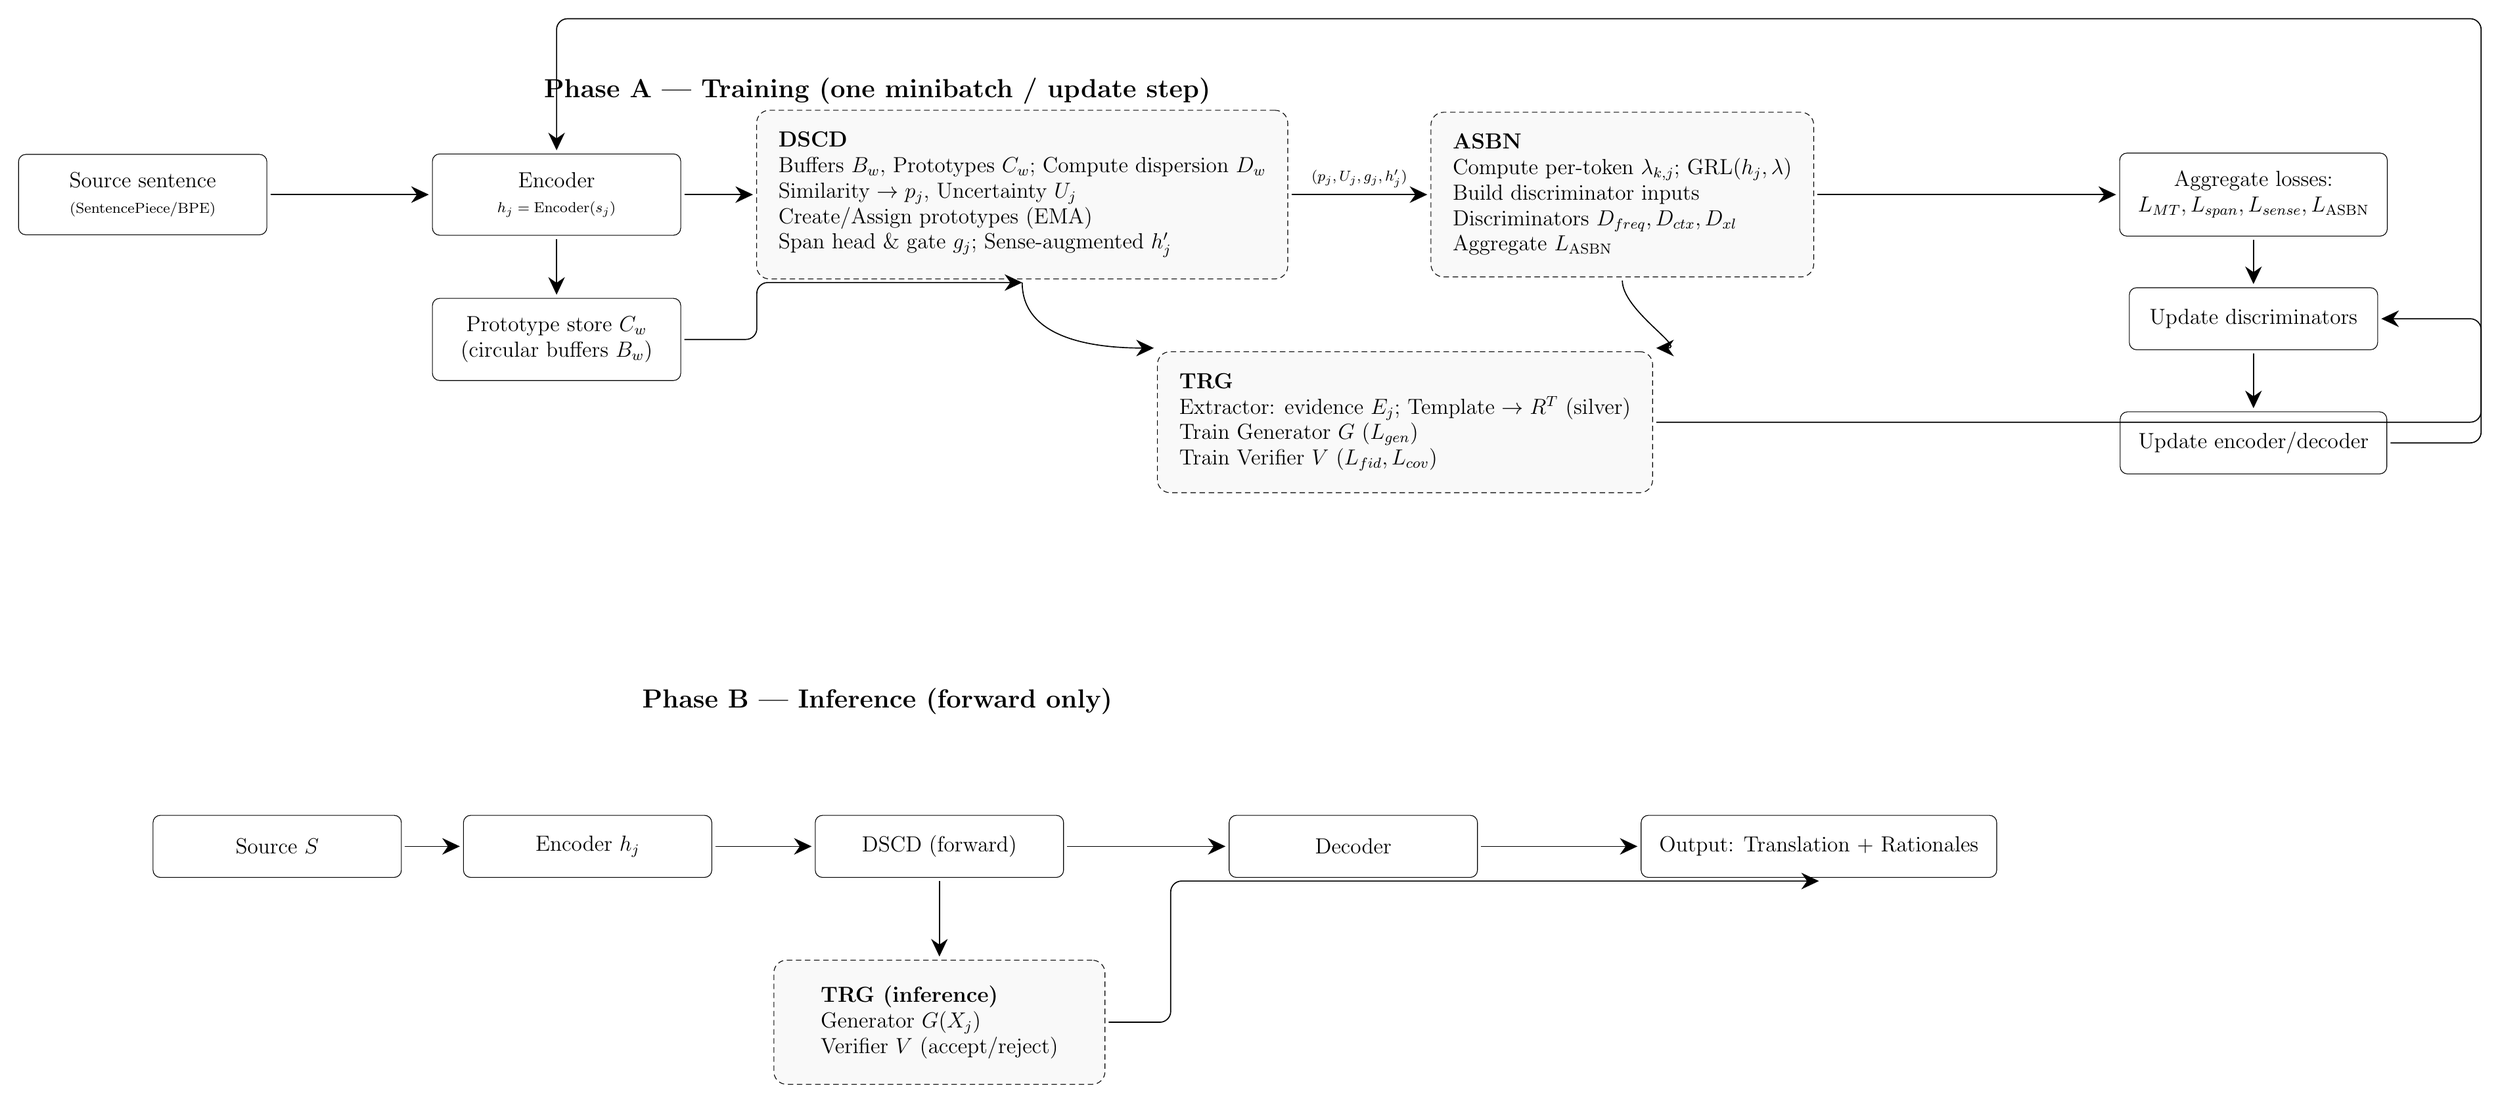
\begin{tikzpicture}[
  every node/.style={font=\large},
  box/.style={
    draw,
    rounded corners=4pt,
    inner sep=10pt,
    align=center,
    minimum width=48mm,
    minimum height=12mm,
    fill=white,
    outer sep=2pt
  },
  module/.style={
    draw,
    rounded corners=7pt,
    densely dashed,
    inner sep=12pt,
    align=left,
    minimum width=64mm,
    minimum height=24mm,
    fill=gray!5,
    outer sep=2pt
  },
  % IMPORTANT: no shorten so arrows reach the node border exactly
  arrow/.style={
    -{Stealth[length=3.4mm,width=3.2mm]},
    semithick,
    rounded corners=6pt
  },
  phaseTitle/.style={font=\Large\bfseries, align=center}
]

% ------------------------------------------------
% Absolute placement with clear routing lanes
% ------------------------------------------------

% Phase A title
\node[phaseTitle] at (0,9.8) {Phase A — Training (one minibatch / update step)};

% Top row (Phase A)
\node[box] (input)  at (-14.2,7.8) {Source sentence \\ \footnotesize (SentencePiece/BPE)};
\node[box] (encoder) at (-6.2,7.8) {Encoder \\ \footnotesize $h_j=\mathrm{Encoder}(s_j)$};

\node[module] (dscd) at (2.8,7.8) {
  \textbf{DSCD}\\
  Buffers $B_w$, Prototypes $C_w$; Compute dispersion $D_w$\\
  Similarity $\to p_j$, Uncertainty $U_j$\\
  Create/Assign prototypes (EMA)\\
  Span head \& gate $g_j$; Sense-augmented $h'_j$
};

\node[module] (asbn) at (14.4,7.8) {
  \textbf{ASBN}\\
  Compute per-token $\lambda_{k,j}$; GRL$(h_j,\lambda)$\\
  Build discriminator inputs\\
  Discriminators $D_{freq}, D_{ctx}, D_{xl}$\\
  Aggregate $L_{\text{ASBN}}$
};

\node[box] (losses) at (26.6,7.8) {Aggregate losses:\\ $L_{MT}, L_{span}, L_{sense}, L_{\text{ASBN}}$};
\node[box] (updDisc) at (26.6,5.4) {Update discriminators};
\node[box] (updEnc)  at (26.6,3.0) {Update encoder/decoder};

% Lower items (Phase A)
\node[box] (prot) at (-6.2,5.0) {Prototype store $C_w$\\(circular buffers $B_w$)};

\node[module] (trg) at (10.2,3.4) {
  \textbf{TRG}\\
  Extractor: evidence $E_j$; Template $\to R^T$ (silver)\\
  Train Generator $G$ ($L_{gen}$)\\
  Train Verifier $V$ ($L_{fid}, L_{cov}$)
};

% Routing lanes (hidden helpers)
\coordinate (topLaneA)   at (29.8,11.2);   % high lane above Phase A
\coordinate (rightLaneA) at (31.0,0.0);    % right vertical lane, clear of boxes

% ------------------------------------------------
% Arrows — Phase A (no overlaps; all arrows reach targets)
% ------------------------------------------------

% Straight top row
\draw[arrow] (input.east) -- (encoder.west);
\draw[arrow] (encoder.east) -- (dscd.west);
\draw[arrow] (dscd.east) -- node[pos=0.5,above]{\footnotesize ($p_j,U_j,g_j,h'_j$)} (asbn.west);
\draw[arrow] (asbn.east) -- (losses.west);

% Losses -> updates
\draw[arrow] (losses.south) -- (updDisc.north);
\draw[arrow] (updDisc.south) -- (updEnc.north);

% updEnc -> encoder (around the outside, no crossings)
\draw[arrow]
  (updEnc.east) -- (rightLaneA |- updEnc.east)
  -- (rightLaneA |- topLaneA)
  -- ($(encoder.north |- topLaneA)$)
  -- (encoder.north);

% Encoder -> Prototype store (vertical)
\draw[arrow] (encoder.south) -- (prot.north);

% Prototype store -> DSCD (enter from bottom-left, avoiding boxes)
\draw[arrow]
  (prot.east) -- ++(14mm,0)
  |- ([xshift=-10mm]dscd.south)
  -- (dscd.south);

% DSCD -> TRG (left entry)
\draw[arrow]
  (dscd.south) to[out=-90,in=180] (trg.north west);

% ASBN -> TRG (right entry, bend outside DSCD)
\draw[arrow]
  (asbn.south) to[out=-90,in=0] (trg.north east);

% TRG -> Update discriminators (go to right lane, then up)
\draw[arrow]
  (trg.east) -- ++(18mm,0)
  -- (rightLaneA |- trg.east)
  -- (rightLaneA |- updDisc.east)
  -- (updDisc.east);

% ------------------------------------------------
% Phase B
% ------------------------------------------------
\node[phaseTitle] at (0,-2.0) {Phase B — Inference (forward only)};

\node[box] (inB)  at (-11.6,-4.8) {Source $S$};
\node[box] (encB) at (-5.6,-4.8) {Encoder $h_j$};
\node[box] (dscdB) at (1.2,-4.8) {DSCD (forward)};
\node[box] (decB)  at (9.2,-4.8) {Decoder};
\node[box] (outB)  at (18.2,-4.8) {Output: Translation + Rationales};

\node[module] (trgB) at (1.2,-8.2) {
  \textbf{TRG (inference)}\\
  Generator $G(X_j)$\\
  Verifier $V$ (accept/reject)
};

% Arrows — Phase B (kept clean and connected)
\draw[arrow] (inB.east) -- (encB.west);
\draw[arrow] (encB.east) -- (dscdB.west);
\draw[arrow] (dscdB.east) -- (decB.west);
\draw[arrow] (decB.east) -- (outB.west);

\draw[arrow] (dscdB.south) -- (trgB.north);
\draw[arrow] (trgB.east) -- ++(12mm,0) |- (outB.south);

\end{tikzpicture}
}
\caption{Landscape-mode TATN diagram with larger boxes and font. Arrows are routed via top and right lanes to avoid overlap and terminate exactly at their target blocks.}
\label{fig:tatn-landscape}
\end{figure}
\end{landscape}




\section{Implementation checklist (practical)}
\begin{itemize}
  \item \textbf{Data preprocessing:} SentencePiece/BPE model; token-level mapping to surface types $w$; optional morphological analyzers for languages like Bengali.
  \item \textbf{Model components:}
    \begin{itemize}
      \item Encoder/Decoder (Transformer-based recommended).
      \item DSCD: circular buffers $B_w$, prototype store $C_w$, $\sigma$-Net (MLP), span head.
      \item ASBN: small MLP discriminators, GRL wrapper with per-token strength.
      \item TRG: small seq2seq generator $G$ and verifier classifier $V$.
    \end{itemize}
  \item \textbf{Key hyperparameters:} $T\in[0.6,1.0]$, $M=3$--8, $\eta\approx0.03$--0.08, $N_{\min}=3$--10, $K_{\max}\approx20$, $\bar\lambda_{\text{freq}}=1.0$, $\bar\lambda_{\text{ctx}}=0.5$, $\bar\lambda_{\text{xl}}=0.8$, $\lambda_{\max}\approx1.0$--2.0.
  \item \textbf{Training schedule:} optional DSCD warmup 1-3 epochs; enable ASBN afterwards; TRG silver collection runs each epoch (or each few batches).
  \item \textbf{Monitoring:} prototype count & creation rate, discriminator training accuracy (should be non-trivial), U histograms, TRG acceptance rate, BLEU/COMET on flagged subsets.
\end{itemize}

\section{Conclusion}
TATN integrates DSCD, ASBN, and TRG to address homograph disambiguation by (1) explicitly modeling candidate senses and uncertainty, (2) removing shortcut signals through targeted adversarial training, and (3) producing verified rationales to make disambiguations transparent and to bootstrap further learning. For low-resource languages (e.g., Bengali $\rightarrow$ English) the modular design is especially valuable: DSCD builds online sense anchors, ASBN prevents frequency-driven errors, and TRG provides human-interpretable explanations that can be inspected or used for weak supervision.



\end{document}
